%%%%%%%%%%%%%%%%%%%%%%%%%%%%%%%%%%%%%%%%%%%%%%%%%%%%%%%%%%%%%%%%%%%%%%%%%%%%%%%%%%%%%%%%%
%  CAPÍTULO 2
%  Referencias:
%    - https://veripool.org/ftp/verilator_doc.pdf
%    - https://zipcpu.com/tutorial/lsn-01-wires.pdf
%%%%%%%%%%%%%%%%%%%%%%%%%%%%%%%%%%%%%%%%%%%%%%%%%%%%%%%%%%%%%%%%%%%%%%%%%%%%%%%%%%%%%%%%%
\chapter{Ejemplos de uso}\label{cap:ejemplos}

%%%%%%%%%%%%%%%%%%%%%%%%%%%%%%%%%%%%%%%%%%%%%%%%%%%%%%%%%%%%%%%%%%%%%%%%
%  Sección 2.1 - Ejemplo básico
%%%%%%%%%%%%%%%%%%%%%%%%%%%%%%%%%%%%%%%%%%%%%%%%%%%%%%%%%%%%%%%%%%%%%%%%
\section{Ejemplo básico}\label{sec:basico}
Como primer ejemplo, vamos a diseñar un módulo con una interfaz muy simple consistente en una entrada y una salida. Lo que hará dicho módulo por dentro será negar la entrada de un bit y conectarla a la salida de un bit. El código, que llamaremos \verb|basico.sv|, será el mostrado en el listing \ref{lst:ejemplo-basico.sv}.

\lstinputlisting[style=verilogstyle, label=lst:ejemplo-basico.sv, caption=Inversor]{codigo/ejemplo-basico/top.sv}

% Subsección 2.1.1 - verilar
\subsection{Verilar}
El primer paso es verilar el modelo. Para ello, ejecutamos la instrucción mostrada en el Listing \ref{lst:verilar} en la raíz del proyecto.

\begin{mycode}[style=bashstyle, label=lst:verilar, caption={Instrucción para verilar el diseño.}]
verilator -Wall -cc inversor.sv
\end{mycode}

\vspace{10pt}
Como se puede ver, se han añadido algunas opciones a la instrucción:

\begin{itemize}
	\item \verb|-Wall|: Activa todos los warnings de sintaxis.
	\item \verb|-cc|: Se verila el diseño en C++ en vez de en SystemC. 
\end{itemize}

Tras esto, hay que hacer un \verb|make| para generar los ficheros objetos asociados al modelo verilado y que luego habrá que enlazar durante la fase de compilación del banco de pruebas. La instrucción es la mostrada en el Listing \ref{lst:make-objects}. Con la opción \verb|-C| indicamos a la instrucción \verb|make| que cambie de directorio durante su ejecución, mientras que con la opción \verb|-f| le indicamos el fichero que tiene que utilizar dentro de dicha ubicación.

\begin{mycode}[style=bashstyle, label=lst:make-objects, caption={Construcción de los ficheros objeto.}]
make -C obj_dir -f Vtop.mk
\end{mycode}

% Subsección 2.1.2 - envolver 
\subsection{Envolver}
El siguiente paso es escribir un banco de pruebas (\textit{testbench} en inglés) en C++ que instancie el modelo verilado y lo inyecte las señales de entrada para verificar que el diseño funciona como debe. Dicho banco de pruebas se suele llamar igual que el fichero fuente del módulo principal, pero añadiéndole el prefijo \verb|tb_|. Por lo tanto, a nuestro banco de pruebas lo llamaremos \verb|tb_inversor.cpp|, y será el que se muestra en el Listing \ref{lst:tb-ejemplo-basico}. En este código se pueden destacar una serie de puntos. El primero es la inclusión de los ficheros de cabecera que contendrán los objetos y funciones necesarios para llevar a cabo la simulación. Estos son \verb|verilated.h|y \verb|Vtop.h|. Este último es uno de los ficheros generados al verilar el modelo en el paso anterior y contiene la declaración de las variables y funciones del modelo verilado (que en C++ pasará a ser una clase), por lo que su nombre dependerá de aquel que le hayamos dado al fichero fuente. El siguiente punto importante es la línea 17, punto en el cual se inicia el contexto de la simulación. Sin entrar mucho en detalle, el contexto se encargará de contener toda la información importante relativa a la simulación, como el tiempo de simulación, entre otras cosas. Además, después se instancia de igual manera un objeto del modelo verilado. En la línea 27 comienza la lógica de la simulación. Esta consiste, en este caso, de un bucle que se ejecutará un número limitado de veces y dentro del cual estimularemos las señales de entrada del modelo verilado con diferentes valoresa lo largo de las diferentes iteraciones del bucle. Asimismo, tras estimular las señales de entrada, llevaremos a cabo una evaluación del sistema en dicho punto (véase la línea 47), es decir, el modelo actualizará los valores de las señales de salida conforme a los de entrada. Tras la evaluación, se muestran los valores de las diferentes señales en la línea 50. Por último, y tras terminar el bucle, liberamos el objeto del modelo verilado.

\lstinputlisting[style=verilogstyle, label=lst:tb-ejemplo-basico, caption={Banco de pruebas del ejemplo básico.}]{codigo/ejemplo-basico/tb_top.cpp}

% Subsección 2.1.3 - compilar 
\subsection{Compilar}
Una vez escrito el banco de prueba hay que compilarlo (véase el Listing \ref{lst:compilar-tb}). Durante la compilación es necesario incluir una serie de directorios que contienen los ficheros necesarios para que la simulación funcione. Por ejemplo, el fichero de cabecera \verb|verilated.h| que incluimos en el banco de pruebas no se encuentra en el directorio estándar de bibliotecas de C, así que hay que incluirlo mediante la opción \linebreak\verb|-I /usr/share/verilator/include/|. Lo mismo ocurre con el directorio \verb|obj_dir|. Por otro lado, el fichero correspondiente al banco de pruebas no va a ser el único fichero fuente que vamos a compilar. Por ejemplo, las funciones declaradas en el fichero de cabecera \verb|verilated.h| están definidas en el fichero \verb|verilated.cpp|, localizado en el mismo directorio que aquel, y que no está compilado por defecto. Por eso es por lo que hay que compilar este y el fichero \verb|verilated_threads.cpp| también.

\begin{mycode}[style=bashstyle, label=lst:compilar-tb, caption={Compilación del banco de pruebas.}]
g++ -I /usr/share/verilator/include/ -I obj_dir/ /usr/share/verilator/include/verilated_threads.cpp /usr/share/verilator/include/verilated.cpp tb_top.cpp obj_dir/Vtop__ALL.a -o Vtop
\end{mycode}

% Subsección 2.1.4 - simular 
\subsection{Simular}
Tras compilar se genera un fichero ejecutable que se puede ejecutar con la orden \verb|./Vtop|. Dicha ejecución crea una salida en la que se muestran los valores de las diferentes señales para cada evaluación del modelo. También podemos redirigir la salida de la simulación a un fichero para su visualización más detenida, en caso de que se quiera ejecutar la simulación durante una cantidad de pasos demasiado alta. La ejecuión del programa mostraría algo como el Listing \ref{lst:salida-ejemplo-basico}.

\lstinputlisting[style=bashstyle, label=lst:salida-ejemplo-basico, caption={Resultados de la simulación del ejemplo básico.}]{codigo/ejemplo-basico/salida.txt}

En la salida se puede observar que el diseño funciona como debe. En cada flanco de subida (\verb|clk=0|), la salida \verb|b| es la negación de la entrada \verb|a|.

% Subsección 2.1.5 - depurar 
\subsection{Depurar}
En este ejemplo sencillo se puede comprobar el correcto funcionamiento del diseño simplemente observando los valores de las señales en la salida. Por lo tanto, no es necesario generar trazas para depurar las señales. Se verá cómo hacer esto en ejemplos posteriores.

%%%%%%%%%%%%%%%%%%%%%%%%%%%%%%%%%%%%%%%%%%%%%%%%%%%%%%%%%%%%%%%%%%%%%%%%
%  Sección 2.2 - Ejemplo con trazas
%%%%%%%%%%%%%%%%%%%%%%%%%%%%%%%%%%%%%%%%%%%%%%%%%%%%%%%%%%%%%%%%%%%%%%%%

\section{Ejemplo con trazas}
En este caso, vamos a explicar el uso de una herramienta que puede ser útil a la hora de depurar un circuito, ya que nos permite visualizar el diagrama de ondas de las señales. Tal vez para este ejemplo tan pequeño, la depuración por este medio puede no ser la más rápida, pero nos permitira ilustrar fácilmente su funcionamiento. En este caso, vamos a diseñar un multiplexor que envíe a la salida una de entre cuatro entradas, es decir, un mux 4:1. El código se muestra en el listing \ref{lst:ejemplo-con-traza}.

\lstinputlisting[style=verilogstyle, label=lst:ejemplo-con-traza, caption={Multiplexor 4 a 1.}]{codigo/ejemplo-con-traza/top.sv}

% Subsección 2.2.1 - verilar 
\subsection{Verilar}
La verilación del circuito es igual que en el ejemplo básico exceptuando la adición de la opción \verb|--trace| que creará el código en C++ necesario para la generación de diagramas de ondas. El comando a ejecutar se muestra en el Listing \ref{lst:verilar-traza}.

\begin{mycode}[style=bashstyle, label=lst:verilar-traza, caption={Instrucción para verilar el diseño habilitando las trazas.}]
verilator -Wall --trace -cc inversor.sv
\end{mycode}

% Subsección 2.2.2 - envolver 
\subsection{Envolver}
La idea a seguir a la hora de programar el banco de pruebas es la misma que en el caso anterior (y en todos los casos): crear una función \verb|main| dentro de la cual programaremos un bucle que estimule el modelo verilado y lo evalue en cada flanco de subida del reloj. No obstante, para crear el fichero con la información necesaria para visualizar el diagrama de ondas hay que instanciar un objeto concreto que nos permitirá volcar la información en dicho fichero. 

En el Listing \ref{lst:tb-ejemplo-con-traza}, se puede ver como, tras la instanciación del modelo verilado, instanciamos el objeto \verb|VerilatedVcdC| llamándolo \verb|tfp| (nótese que hay que incluir el fichero de cabecera correspondiente al principio), y que contiene las funciones necesarias para la creación del fichero que abriremos con un programa de visualización de diagramas de ondas (GTKWave) y para el volcado del estado de las señales en dicho fichero. En la línea 34, pasamos dicho objeto a la función \verb|trace| del modelo verilado, de manera que este quede asociado a dicho modelo y trace sus señales. El 99 indica los niveles de jerarquía que queremos trazar. Cada nivel se corresponde con la instanciación de un módulo dentro del módulo que se quiere trazar, de tal modo que si el módulo \verb|top.sv| instancia un módulo \verb|m1.sv| y este a su vez un módulo \verb|m2.sv|, la jerarquía tendrá 2 niveles. Con un valor de 99 nos aseguramos de que todas las señales del circuito se tracen, ya que es muy difícil que un diseño tenga tantos niveles de jerarquía. En la línea 35, utilizamos el objeto \verb|tfp| para abrir el fichero en el que volcaremos los datos de las señales durante la simulación. La ruta que se le pasa entre paréntesis es relativa, de tal manera que dicho fichero se guardará en el directorio donde se encuentre el banco de pruebas. Para volcar los datos de las señales en un momento dado, se usa la función \verb|dump| del objeto \verb|tfp|. Para indicar el tiempo de simulación que queremos volcar, pasamos el valor devuelto por la función \verb|time| del contexto de la simulación. Finalmente, antes de liberar el modelo verilado, cerramos el fichero con los datos de los diagramas de ondas (línea 74).

\begin{center}
	\lstinputlisting[style=verilogstyle, label=lst:tb-ejemplo-con-traza, caption={Banco de pruebas para el ejemplo con traza.}]{codigo/ejemplo-con-traza/tb_top.cpp}
\end{center}


% Subsección 2.2.3 - compilar 
\subsection{Compilar}
La compilación del banco de pruebas es muy similar también al ejemplo básico, pero incluyendo un fichero nuevo que hay que compilar. El fichero extra que hay que compilar es el que implementa las funciones indicadas en el fichero de cabecera que incluimos en el banco de pruebas: \verb|verilated_vcd_c.h|. Si se ha instalado Verilator de la manera estándar, dicho fichero se debería encontrar en \linebreak\verb|/usr/share/verilator/include/verilated_vcd_c.cpp|. De este modo, el comando para compilar quedaría de la manera que se muestra en el Listing \ref{lst:compilar-tb-traza}.

\begin{mycode}[style=bashstyle, label=lst:compilar-tb-traza, caption={Compilación del banco de pruebas incluyendo el fichero necesario para crear trazas.}]
g++ -I /usr/share/verilator/include/ -I obj_dir/ /usr/share/verilator/include/verilated_threads.cpp /usr/share/verilator/include/verilated.cpp /usr/share/verilator/include/verilated_vcd_c.cpp tb_top.cpp obj_dir/Vtop__ALL.a -o Vtop
\end{mycode}

% Subsección 2.2.4 - simular 
\subsection{Simular}
Si la compilación es exitosa, se debería crear el ejecutable \verb|Vtop| que, tras su ejecución, debería mostrar en la salida estandar los resultados de la simulación y generar un fichero llamado \verb|simx.vcd| y que es el que utilizaremos abriremos con el programa GTKWave para visualizar el diagrama de ondas.

% Subsección 2.2.5 - depurar 
\subsection{Depurar}
Para depurar de una manera más visual, o seleccionar sólo un subconjunto del total de señales del circuito, vamos a utilizar el visualizador de diagramas de ondas GTKWave. Dicho programa se lanza desde la terminal, pasándole como argumento el fichero \verb|.vcd| que hemos generado durante la simulación (véase el Listing \ref{lst:depurar}).

\begin{mycode}[style=bashstyle, label=lst:depurar, caption={Instrucción para lanzar el programa de visualización de diagramas de ondas.}]
gtkwave simx.vcd
\end{mycode}

En la Figura \ref{fig:gtkwave-ejemplo-con-traza} se muestra el programa en ejecución. En él se han seleccionado todas las señales del circuito y se han insertado en el panel principal para su visualización.

\begin{figure}[htb]
	\centering
	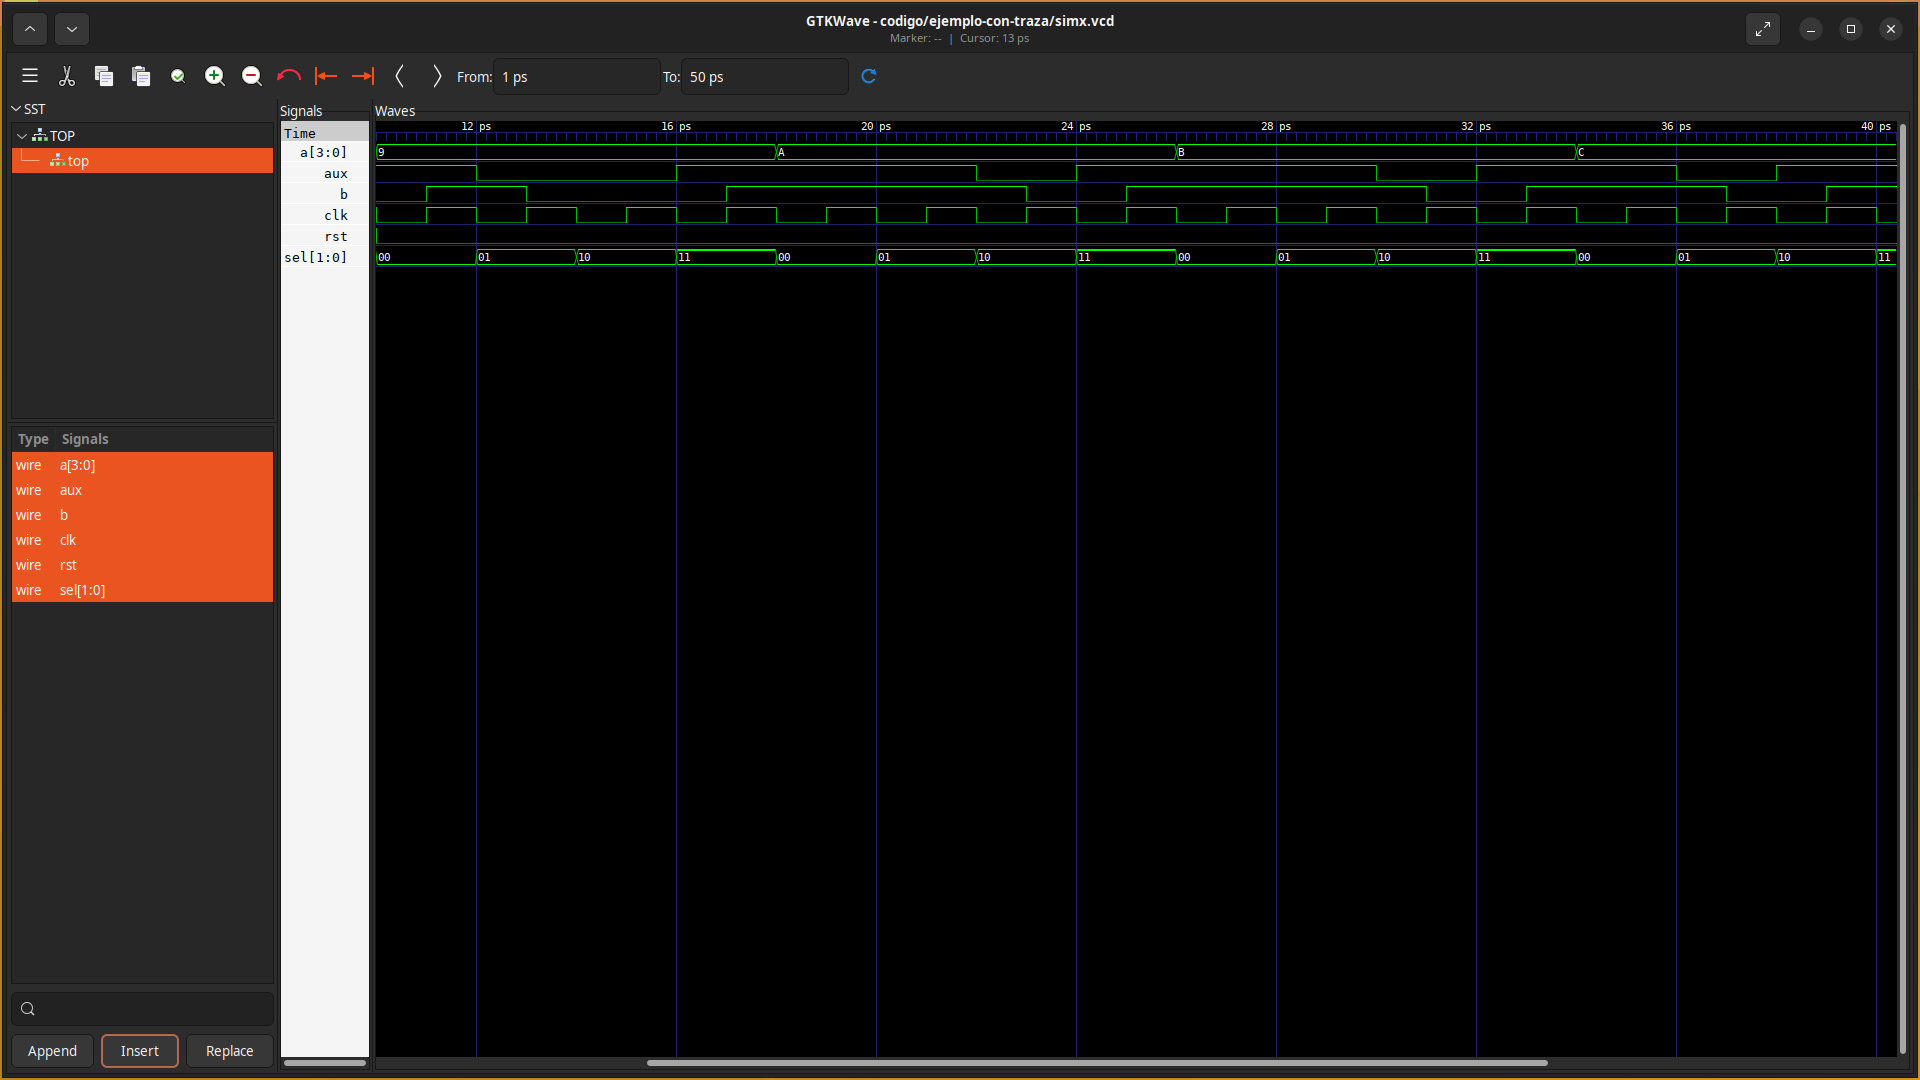
\includegraphics[width=\textwidth]{figs/gtkwave-ejemplo-con-traza.png}
	\caption{GTKWave.}
	\label{fig:gtkwave-ejemplo-con-traza}
\end{figure}
